\section{Long period comparison}
\label{sect:lts_study}

% ----------------------
% Introduction / aims etc
% ----------------------
\subsection{Introduction and aims}
This study is aimed at comparing the effectiveness of different scheduling algorithms and configurations of scheduling algorithms under varying conditions. In particular the effectiveness of schedulers under varying load and environmental stability. In order to make these comparisons it is neccessary to develop generators to create phase2 models with specific load characteristics and environmental models with specific stability criteria in order to have an independant variable to 


% ----------------------
% Env Scenarios
% ----------------------
\subsection{Variable environmental models}
- context of stability 
From Section (XXX) we see that the environmental conditions at the telescope site (specifically seeing) are seen to vary over different timescales from minutes to hours. The seeing conditions are split into several bands defined as: (G) good (s < 0.8''), (A) average ($0.8'' < s <= 1.3''$), (P) poor ($1.3'' < s <= 3.0''$) , (U) usable ($3'' < s <= 5''$), (B) bad/unusable ($s > 5''$). From the point of view of scheduling it is only these bands which matter. So long as the seeing varies within any band, neither contention or scoring of groups are affected. When the seeing transitions between bands both are affected. 

From a defined set of E model parameters we can generate any number of E scenarios (effectively instantiations of the model) - it would be useful to see if we get variation in results and indeed in the SQMs from different scenarios generated by the same model - if this variation is large we will have to run many more simulations and there will be x-errors in addition to the expected y-errors.

\subsubsection{Modelling seeing variation}
Seeing variation can be modelled by a simple transition matrix $P(t)$ where each element $P_{ij}(t)$ represents the cumulative probability of transitioning from state i to state j within a period t. The diagonal elements $P_{ii}(t)$ represent the probability of \emph{remaining} in a particular state for time upto t. 
\begin{equation}
 \left( 
\begin{array}{ccccc}
  P_{gg}(t) & P_{ga}(t) & P_{gp}(t) & P_{gu}(t) & P_{gb}(t)\\
  P_{ag}(t) & P_{aa}(t) & P_{ap}(t) & P_{au}(t) & P_{ab}(t)\\
  P_{pg}(t) & P_{pa}(t) & P_{pp}(t) & P_{gu}(t) & P_{pb}(t)\\
  P_{ug}(t) & P_{ua}(t) & P_{up}(t) & P_{uu}(t) & P_{ub}(t)\\
  P_{bg}(t) & P_{ba}(t) & P_{bp}(t) & P_{bu}(t) & P_{bb}(t)

\end{array} 
\right)
\end{equation}

 The relative distribution of time spent in each band is of little interest from the point of view of these studies - only the stability or frequency of change is important.  The diagonal elements were therefore set to the same value based on a stability parameter $\tau_E$ such that the probability of remaining in a given band/state for upto time t is given by $P_{ii}(t) = 1 - \exp{t/\tau_E}$. The Bad and usable bands are also of less interest - bad indicates no observing possible, and in practice relatively few groups are ever setup with such lax seeing constraints consequently the array is reduced to 3x3. The non-diagonal elements are each set to the same value, namely $P_{ij} = 0.5*(1 - P_{ii}$` . 


A specific seeing scenario is generated by taking random intervals calculated from $-\tau_E \ln{(1-R)}$ where R is a random number in $[0,1]$. At each period the seeing is allowed to change randomly to another value (band) - we are not particularly bothered which value or how the time spent in the different bands is distributed only that it is changing.

\subsubsection{Environmental Model Generator study}
. Results of a run with $\tau_E =30 mins$ are shown in Fig.~\ref{fig:env_profile_18} which shows an actual seeing scenario over a period of 7 days for this $E_{1800}$ model (1800 sec = 30 min). Fig.~\ref{fig:env_comp_18} shows a comparison for the relative amounts of time under varying lengths of stability period for several runs of the $E_{1800}$ model generator. We see from this that the models are generally quite stable i.e. that a given control parameter $\tau_E$ gives consistent results in terms of the distribution of lengths of stable periods. Fig.~\ref{fig:env_relstats} and  Fig.~\ref{fig:env_cumstats} show the relative and cumulative distribution of lengths of periods of stability for various models with $\tau_E$ running from 30 minutes to 4 hours over scenario runs of 100 days.


\begin{figure}[h]
\begin{center}
 \includegraphics[scale=0.5, angle=-90]{figures/e_18_prof.eps}
\end{center} 
 \caption[Environmental scenario (7 day snapshot).] 
   {Long period study. 7 day snapshot of generated environmental scenario $E_{1800}$.}
\label{fig:env_profile_18}
\end{figure}


\begin{figure}[h]
\begin{center}
 \includegraphics[scale=0.5, angle=-90]{figures/e_18_comp.eps}
 \caption[Environmental scenario - comparison between runs of $E_{1800}$] 
   {Long period study. Comparison of relative amounts of time in periods of stability for several runs of $E_{1800}$.}
\label{fig:env_comp_18}
\end{center} 
\end{figure}

\begin{figure}[h]
\begin{center}
 \includegraphics[scale=0.5, angle=-90]{figures/e_relstats.eps}
 \caption[Environmental scenario - relative distribution of stable period lengths.] 
   {Long period study. Relative distribution - number of periods with stability in variable range.}
\label{fig:env_relstats}
\end{center} 
\end{figure}

\begin{figure}[h]
\begin{center}
 \includegraphics[scale=0.5, angle=-90]{figures/e_cumstats.eps}
 \caption[Environmental scenario - cumulative distribution of stable period lengths.] 
   {Long period study. Cumulative distribution - total time where stability upto variable range.}
\label{fig:env_cumstats}
\end{center} 
\end{figure}

\subsubsection{Summary and conclusions}
ESG generates consistent scenarios wrt stability characteristic - good indepenent var.



% ----------------------
% Phase2 Generators
% ----------------------
\subsection{Phase 2 model charcaterisation}
Before embarking on any scheduler comparisions there is a need to decide which type of phase II model to use. A real model suffers from the ODB evolution problem (see \ref{XXX}). With a generated model however, group activations are spread out over a specified period (say several months) so new groups are appearing in the schedule every day - like the real ODB but in that case they are typically not entered until just before required so using daily snapshots, we do not know about them in advance and cannot take them into account easily.
   

Additionally, it would be useful to see if different schedulers perform better than others when faced with phase2 models (pools of observation requests) with different \emph{weight} or \emph{load} characteristics.  i.e. is one scheduler better at handling \emph{light} loading and another better at handling \emph{heavy} loading.

\subsubsection{Which PCM to use to characterise a phase2 model} 
We have seen from Sect.(XXX) that there are several complexity metrics (PCMs) available. None of these are able to fully characterize the loading as this varies through the night and from day to day and is dependant on what has (or might have) occurred previously. Of the serveral contenders, the average contention $C_C$ was chosen. This is a metric which is easy to calculate and readily visualized.
 
\subsubsection{how generate models - ref annex for params} 
A Phase2 Model generator was designed to create phase2 models with varying characteristics. This generator, described in Appendix (XX) has a large number of configurable parameters. 


Results for 4 generated models $P_l$ - $P_h$ are shown in figures \ref{fig:c60_gen_av} and \ref{fig:c60_gen_ng}. Similar figures for the ODB snapshots though on a different scale (what does that mean?) are shown in \ref{fig:c60_odb_av} and \ref{fig:c60_odb_ng}.

\begin{figure}[h]
\begin{center}
 \subfigure[Variation of average contention $\bar{C_c}$ for generated phase2 models.] {
   \label{fig:c60_gen_av}
   \includegraphics[scale=0.5, angle=-90]{figures/c60_gen_cav.eps}
  }
 \subfigure[Variation of number of executed groups for generated phase2 models.] {
   \label{fig:c60_gen_ng}
   \includegraphics[scale=0.5, angle=-90]{figures/c60_gen_ng.eps}
  }
 \end{center}
\end{figure}

\begin{figure}[h]
\begin{center}
 \subfigure[Variation of average contention $\bar{C_c}$ for ODB snapshots.] {
   \label{fig:c60_odb_av}
   \includegraphics[scale=0.5, angle=-90]{figures/c60_odb_cav.eps}
  }
 \subfigure[Variation of number of executed groups for ODB snapshots.] {
   \label{fig:c60_odb_ng}
   \includegraphics[scale=0.5, angle=-90]{figures/c60_odb_ng.eps}
  }
\caption{Comparison of average contention measure and number of groups executed per night for generated phase2 models and ODB snapshots.}
 \end{center}
\end{figure}



It is however not possible to easily generate a specific phase2 model instance with a specific set of PCM characteristics. Consequently in order to explore a range of these characteristics it is neccessary to generate a number of different models from the same generator and then measure the characteristic of that model.

\subsubsection{Characterisation study}
A set of 4 model generators were chosen and are described in more detail in Table.~\ref{tab:ltc_p2models}. These generators are selected to represent a range of charcateristics from light (designed to create low-load phase2 models) upto heavy (designed to generate high load models). A series of tests were performed using XX models generated by each generator. The models were characterised in terms of the chosen PCM - the average contention ($C_C$). A series of simulations were performed on each model to generate a set of SQMs (specifically $Q_{SU}$ - a score based metric and $Q_{XT}$ - the fraction of night observed. 

From a given generator model (e.g. $P_l$) we can generate any number of actual instances - ideally these would all have the same measurable characteristics (e.g. $\bar{C_c}$) but this is not guaranteed. Tests were run using each of the generator models in order to determine the variation of characteristics. The measurable characteristic chosen was $\bar{C_{dc}}$ - the average dynamic contention over the measurment period. A simple scheduler was chosen using best-score selection and a single $f_{OH}$ metric - i.e. the target which was highest relative to maximum attainable elevation was chosen at each sweep. We are not interested in the scheduler here, only the variability of the generated  P2 characteristics. Simulations were run for the middle 30 days () of the generated models and the values of $\bar{Q_{SU}}$ and $\bar{Q_{XT}}$ are plotted against $\bar{C_c}$ for each model. The results are shown in Fig.~\ref{fig:p2_gen_su} and  Fig.~\ref{fig:p2_gen_xt}.



\begin{figure}[h]
\begin{center}
 \includegraphics[scale=0.5, angle=-90]{figures/p2_gen_qsu.eps}
 \caption[Variation of $Q_{SU}$ with $C_C$ for variable phase2 generator models.] 
   {Variation of $Q_{SU}$ with $C_c$. Each point represents a single phase 2 model generated by one of 4 initial sets of generators.}
\label{fig:p2_gen_su}
\end{center}
\end{figure}


\begin{figure}[h]

\begin{center}
 \includegraphics[scale=0.5, angle=-90]{figures/p2_gen_qxt.eps}
 \caption[Variation of $Q_{XT}$ with $C_C$ for variable phase2 generator models.] 
   {Variation of $Q_{XT}$ with $C_c$. Each point represents a single phase 2 model generated by one of 4 initial sets of generators.}
\label{fig:p2_gen_xt}
\end{center} 
\end{figure}


\subsubsection{Summary and conclusions}
From the results it is clear there is significant variation in the measurable characteristic for any model though there is a progression between models as might be expected i.e. all the $P_s$ contention values are lower than all the $P_h$ values. There is significant overlap between \emph{adjacent} models. The heavy model generally uses up all or very nearly all of the available night - this is not too surprising - there are more groups to chose from so likely to be few if any slack periods. There is most variation in $Q_{SU}$ for the small models - with low contention there will be periods when no groups are actually schedulable hence the requent depression of this metric.



% ----------------------
% BDS with different z-models
% ----------------------
\subsection{BDS study using various z-models}
Studies of the basic despatch scheduler so far have been based on the \emph{best} selection model $\zeta_{Best}$. This selects the highest scoring group on each sweep and is the intuitive course of action. Some studies by (check refs) have suggested that introducing an element of bias or randomness can sometimes improve overall results. This can be understood in the telescope scheduling domain by the following observations:-
\begin{itemize}
\item Often the top few groups at the end of scoring sweep have similar scores - i.e. there is little to chose between them - if we were to run the sweep a few minutes earlier or later a different group might win. 
\item Selecting any group for execution neccessarily excludes other groups which may not be enabled just at that moment but might be shortly. Selection of a group with a long execution time might occasionally result in exclusion of a more valuable group which is just outside its window of opportunity.
\end{itemize}

If we consider the normal \emph{best} selection technique as a hill-climbing or gradient search over the space of possible solutions, it is well known that such techniques though efficient in regular and simple spaces tend to be sub-optimal in complex search spaces by ``missing the global peaks whilst getting stuck on local peaks''. Randomization allows us to jump of an apparently good ``hillside'' where we are converging on the peak and (possibly) land on the foothills of another higher peak - global optimization versus local optimization.


\begin{description}
\item [Best ranked] $\zeta_{best}$ - The best or highest ranked candidate is selected, representing the local optimization or hill-climbing search.

\item [Fixed rank bias] $\zeta_{FR}$ - Candidates are selected with probability determined by a fixed percentage based on their relative ranking. This is just a general randomization technique. 

\item [Relative score bias] $\zeta_{RS}$ - Candidates are selected with probabality determined by relative scores. This takes account of point (XXX backref) above.
\end{description}

Describe the scoring function weights used which is also Qsu.

\subsubsection{study effect of bias etc}
For this study a basic despatch scheduler (BDS) is setup using a variety of selection models to be tested.
The principle selection models to be used are setup using these parameters:-
best - bfr (80,15,3,2,*) - brs (). A series of simulations are performed using the folllowing scoring model:- describe f weights.

Ensemble plots for each selection model here - qsu v time. Extract average per night for ZB as comparison for bias ensembles to see if they are better/worse on each night.

\begin{figure}[h]

\begin{center}
 \includegraphics[scale=0.5, angle=-90]{figures/best_ensemble.eps}
 \caption[Ensemble plot showing variation of $Q_{SU}$ with time for selection model $\zeta_{Best}$.] 
   {Ensemble plot showing variation of $Q_{SU}$ with time for selection model $\zeta_{Best}$.}
\label{fig:ensemble_best}
\end{center} 
\end{figure}

\begin{figure}[h]
 
\begin{center}
 \includegraphics[scale=0.5, angle=-90]{figures/biasfr_ensemble.eps}
 \caption[Ensemble plot showing variation of $Q_{SU}$ with time for selection model $\zeta_{FR}$.] 
   {Ensemble plot showing variation of $Q_{SU}$ with time for selection model $\zeta_{FR}$.}
\label{fig:ensemble_fixrankbias}
\end{center}
\end{figure}


\begin{figure}[h]

\begin{center}
 \includegraphics[scale=0.5, angle=-90]{figures/biasrs_ensemble.eps}
 \caption[Ensemble plot showing variation of $Q_{SU}$ with time for selection model $\zeta_{RS}$.] 
   {Ensemble plot showing variation of $Q_{SU}$ with time for selection model $\zeta_{RS}$.}
\label{fig:ensemble_relscorebias}
\end{center} 
\end{figure}



\subsubsection{see if e-stab variation}
Test the scheduling selection models under varying environmental stability conditions to see if any model produces an improvment over the standard \emph{best} selection.
Next test is with variable DE ie env model stability. The P model is fixed for this. Note CC value. 


Plots here for qsu v DE

\begin{figure}[h]

\begin{center}
 \includegraphics[scale=0.5, angle=-90]{figures/best_de.eps}
 \caption[Variation of $Q_{SU}$ with $\tau_E$ for selection model $\zeta_{Best}$.] 
   {Variation of $Q_{SU}$ with $\tau_E$ for selection model $\zeta_{Best}$.}
\label{fig:qsu_de_best}
\end{center} 
\end{figure}

\begin{figure}[h]

\begin{center}
 \includegraphics[scale=0.5, angle=-90]{figures/biasfr_de.eps}
 \caption[Variation of $Q_{SU}$ with $\tau_E$ for selection model $\zeta_{FR}$.] 
   {Variation of $Q_{SU}$ with $\tau_E$ for selection model $\zeta_{FR}$.}
\label{fig:qsu_de_biasfr}
\end{center}
 \end{figure}

\begin{figure}[h]

\begin{center}
 \includegraphics[scale=0.5, angle=-90]{figures/biasrs_de.eps}
 \caption[Variation of $Q_{SU}$ with $\tau_E$ for selection model $\zeta_{RS}$.] 
   {Variation of $Q_{SU}$ with $\tau_E$ for selection model $\zeta_{RS}$.}
\label{fig:qsu_de_biasrs}
\end{center}
\end{figure}

\begin{figure}[h]

\begin{center}
 \includegraphics[scale=0.5, angle=-90]{figures/all_de.eps}
 \caption[Effect of selection model on variation of $Q_{SU}$ with $\tau_E$.] 
   {Effect of selection model on variation of $Q_{SU}$ with $\tau_E$.} 
\label{fig:qsu_de_allcomp}
\end{center}
\end{figure}

\subsubsection{Summary/conc}

% ----------------------
% QLAS Study
% ----------------------
\subsection{QLAS study}
\subsubsection{describe QLAS function (see SPIE08)}
\subsubsection{study variation of CC}
\subsubsection{study variation of e-stab}
\subsubsection{Summary/conc}

% ----------------------
% Future stuff
% ----------------------
\subsection{Future work} 
- pull concs from other bits together here
-volatility measure
-adaptive scheduling
- other schedulers - min-energy model
